\documentclass[a4paper]{article}

\usepackage{fullpage} % Package to use full page
\usepackage{parskip} % Package to tweak paragraph skipping
\usepackage{amsmath}
\usepackage{hyperref}
\usepackage{amsmath,amsfonts,amsthm} % Math packages
\usepackage{graphicx}
\usepackage{listings}
\usepackage{color}
\usepackage{float}
\definecolor{codegreen}{rgb}{0,0.6,0}
\definecolor{codegray}{rgb}{0.5,0.5,0.5}
\definecolor{codepurple}{rgb}{0.58,0,0.82}
\definecolor{backcolour}{rgb}{0.95,0.95,0.92}
\definecolor{brown}{rgb}{0.59, 0.29, 0.0}
\definecolor{beaublue}{rgb}{0.74, 0.83, 0.9}
\definecolor{orange}{rgb}{1.0, 0.5, 0.0}
\definecolor{darkslategray}{rgb}{0.18, 0.31, 0.31}
\def\Xint#1{\mathchoice
	{\XXint\displaystyle\textstyle{#1}}%
	{\XXint\textstyle\scriptstyle{#1}}%
	{\XXint\scriptstyle\scriptscriptstyle{#1}}%
	{\XXint\scriptscriptstyle\scriptscriptstyle{#1}}%
	\!\int}
\def\XXint#1#2#3{{\setbox0=\hbox{$#1{#2#3}{\int}$}
		\vcenter{\hbox{$#2#3$}}\kern-.5\wd0}}
\def\dashint{\Xint-}

% Swap the definition of \abs* and \norm*, so that \abs
% and \norm resizes the size of the brackets, and the 
% starred version does not.
\makeatletter
\let\oldabs\abs
\def\abs{\@ifstar{\oldabs}{\oldabs*}}
%
\let\oldnorm\norm
\def\norm{\@ifstar{\oldnorm}{\oldnorm*}}
\makeatother
\lstdefinestyle{mystyle}{
	backgroundcolor=\color{white},   
	commentstyle=\color{codegreen},
	keywordstyle=\color{blue},
	identifierstyle=\color{brown},
	numberstyle=\tiny\color{codegray},
	stringstyle=\color{orange},
	basicstyle=\footnotesize,
	breakatwhitespace=false,         
	breaklines=true,                 
	captionpos=b,                    
	keepspaces=true,                 
	numbers=left,                    
	numbersep=5pt,                  
	showspaces=false,                
	showstringspaces=false,
	showtabs=false,                  
	tabsize=2
}
\lstset{style=mystyle}
\newenvironment{mat}{\left[ \begin{array}{ccccccccccccc}}{\end{array}\right]}

\newcommand\bcm{\begin{mat}}
\newcommand\ecm{\end{mat}}

\title{AMATH 568: Problem Set 2}
\author{Jithin D. George, No. 1622555}
%\date{23/11/16}

\begin{document}

\maketitle
\begin{enumerate}

	
	\item 
\[A = \bcm \lambda &1 &0\\ 0 &\lambda &1\\ 0 &0 &\lambda  \ecm \]
\[A^0 = \bcm 1 &0 &0\\ 0 &1 &0\\ 0 &0 &1  \ecm \]
\[A^2 = \bcm \lambda^2 &2\lambda &1\\ 0 &\lambda^2 &2\lambda\\ 0 &0 &\lambda^2  \ecm \]
\[A^3 = \bcm \lambda^3 &3\lambda^2 &3\lambda\\ 0 &\lambda^3 &3\lambda^2\\ 0 &0 &\lambda^3  \ecm \]
\[A^n = \bcm \lambda^n &n\lambda^{n-1} &\frac{n(n-1)}{2} \lambda^{n-2}\\ 0 &\lambda^n &n\lambda^{n-1}\\ 0 &0 &\lambda^n  \ecm \]

The diagonal elements of $e^{At}$ are of the form
\[1 +\lambda t + \frac{\lambda^2 t^2}{2!}+ \frac{\lambda^3 t^3}{3!} +\ldots = e^{\lambda t}  \]
The  first off-diagonal elements of $e^{At}$ are of the form
\[t + \frac{2 \lambda  t^2}{2!}+ \frac{3\lambda^2 t^3}{3!} +\ldots = f \]
\[1 +\lambda t + \frac{\lambda^2 t^2}{2!}+ \frac{\lambda^3 t^3}{3!} +\ldots = \frac{f}{t}  \]
\[e^{\lambda t}  = \frac{f}{t}  \]
\[f= te^{\lambda t}\]
The  second off-diagonal elements of $e^{At}$ are of the form
\[ \frac{ t^2}{2!}+ \frac{3\lambda t^3}{3!} + \frac{6\lambda^2 t^4}{4!}+\ldots = g \]
\[ \frac{ t^2}{}+ \frac{\lambda t^3}{1} + \frac{\lambda^2 t^4}{2!}+\ldots =2 g \]
\[1 +\lambda t + \frac{\lambda^2 t^2}{2!}+ \frac{\lambda^3 t^3}{3!} +\ldots = \frac{2g}{t^2}  \]
\[e^{\lambda t}  = \frac{2g}{t^2}  \]
\[g= \frac{t^2e^{\lambda t}}{2}\]
\[e^{At} =\bcm \lambda e^{\lambda t} &te^{\lambda t} &\frac{t^2}{2}e^{\lambda t}\\ 0 &e^{\lambda t} &te^{\lambda t}\\ 0 &0 &e^{\lambda t}  \ecm\]


\item
\begin{enumerate}
	\item
	
	We know that,
	\[  \frac{d}{dt} det[\Phi(t)]= det[\Phi(t)] Tr(B)  \]
	
	where
	\[  \Phi B  = A \Phi\]	
	
	\[  \frac{d}{dt} ln( det[\Phi(t)]) = \frac{1}{det[\Phi(t)]} \frac{d}{dt} det\Phi  \]	
	
	\[  = \frac{det[\Phi(t)] Tr(B)}{det[\Phi(t)]}   \]		
	\[  = Tr(B)  \]	
		\[  = Tr(A(t))  \]	
		
\item
\[\Phi'(t+T)= A(t+T)\Phi(t+T)  \]	
\[= A(t)\Phi(t+T)  \]	

So, both $\Phi(t)$ and $\Phi(t +T)$ solve $ x'= Ax $. They are both fundamental matrices. Since they solve a group of linearly independent equations,
\[\Phi(t+T)= \Phi(t)C  \]
 where C is a constant matrix.
 Since $\Phi(0)$ is non-singular, $\Phi(t)$ is too and C is non-singular as well. So, we can find a B such that
 \[C= e^{BT}\]
 Let 
 \[\Phi(t)= e^{Bt} Q(t)\]
 \[ Q(t)= \Phi(t)e^{-B(t)}\]	
  \[ Q(t+T)= \Phi(t+T)e^{-B(t+T)}\]	
    \[ = \Phi(t)e^{BT}e^{-B(t+T)}\]	
        \[ = \Phi(t)e^{Bt} = Q(t)\]
So, Q(t) is periodic. And we have,
 \[\Phi(t)= e^{Bt}Q(t) \]	
\end{enumerate}

\item
\begin{enumerate}
	\item
	 The fixed points are at (0,0), (0,1) , (2,0) and (0.5,1.5)
	 \item The Jacobian is given by
	 \[J*(x,y)= \begin{bmatrix}
	 2-2x-y &-x\\ \frac{y^2}{(1+x)^2} &1-\frac{2y}{1+x}
	 \end{bmatrix}\]
	 At (0,0), 
	 \[J*(0,0)= \begin{bmatrix}
	 2 &0\\ 0 &1
	 \end{bmatrix}\]
	 The eigenvalues are 2 and 1. Since both are positive, this point is unstable.
	 The eigenvectors are (1,0) and (0,1)
	 
	 At (0,1), 
	 \[J*(0,1)= \begin{bmatrix}
	 1 &0\\ 1 &-1
	 \end{bmatrix}\]
	 The eigenvalues are -1 and 1. Since one value has a positive real part, this point is unstable.
	 The eigenvectors are (0,1) and (0.89442719, 0.4472136).	 	 
	
	 At (2,0), 
	 \[J*(2,0)= \begin{bmatrix}
	 -2 &-2\\ 0 &1
	 \end{bmatrix}\]
	 The eigenvalues are -2 and 1. Since one value has a positive real part, this point is unstable.
	 The eigenvectors are (1,0) and (-0.5547002, 0.83205029).
	 
	 At (0.5,1.5), 
	 \[J*(0.5,1.5),= \begin{bmatrix}
	 -0.5 &-0.5\\ 1 &-1
	 \end{bmatrix}\]
	 The eigenvalues are -0.75 +0.6614i and -0.75-0.6614i. Since both values have a negative real part, this point is stable.
	 The eigenvectors are (0.2041 + 0.5401i,0.8165 ) and (0.2041 - 0.5401i, 0.8165 ).	
	 \item Done in part(b)
	 \item 
	 
	 
	 
	    \begin{figure}[H]
	    	\centering
	    	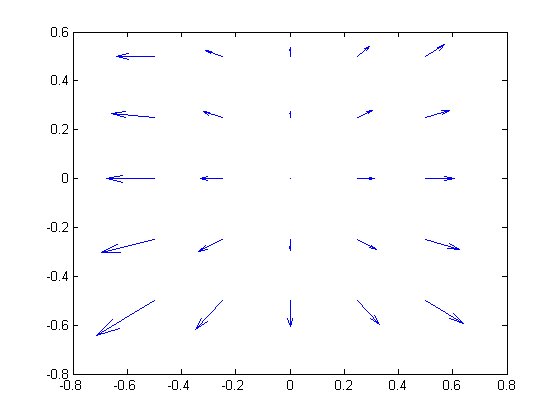
\includegraphics[width=12cm]{zerozero}
	    	\caption{Phase portrait in vicinity of (0,0) }
	   
	    \end{figure}
	    The eigenvectors (1,0) and (0,1) are orthogonal and is well-represented by the stretching in perpendicular directions. 
\begin{figure}[H]
	\centering
	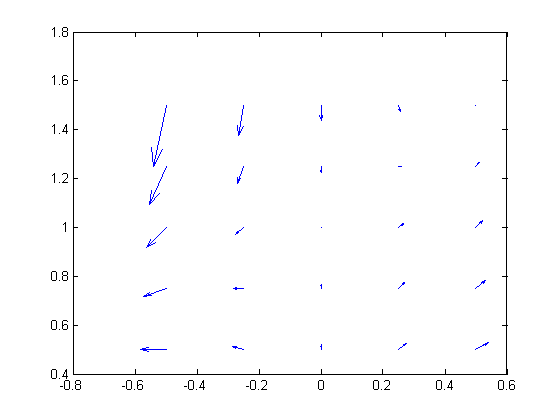
\includegraphics[width=12cm]{zeroone}
	\caption{Phase portrait in vicinity of (0,1) }
\end{figure}
	    The eigenvectors (0,1) corresponds to stretching in the vertical direction.
\begin{figure}[H]
	\centering
	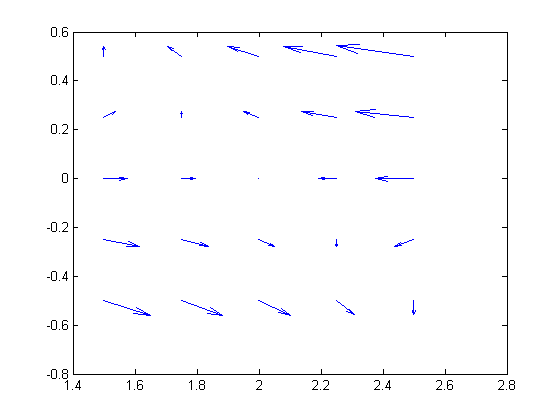
\includegraphics[width=12cm]{two}
	\caption{Phase portrait in vicinity of (2,0) }
\end{figure}
	    The eigenvectors (1,0) represents stretching in the horizontal direction but since the eigenvalue is negative, it is an inward compression.
\begin{figure}[H]
	\centering
	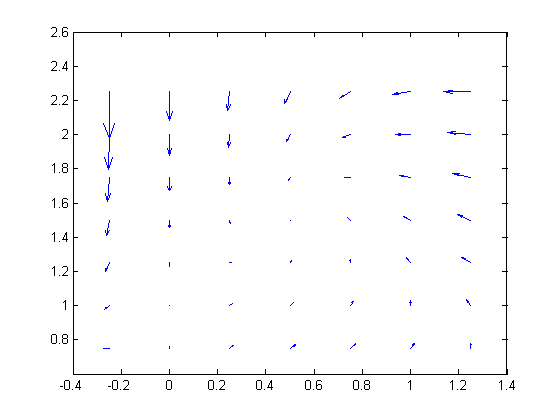
\includegraphics[width=12cm]{half}
	\caption{Phase portrait in vicinity of (0.5,1.5) }
\end{figure}
	    The complex eigenvectors correspond to the spiral.	
The plots were obtained in Matlabd using the following code
\begin{lstlisting}[language=Matlab,frame=single]
clear all; close all; clc;
a=0.5;
b=1.5;
[x,y]=meshgrid(-0.5+a:0.25:a+0.5,-0.5+b:0.25:0.5+b);
xdot=x.*(2-x)-x.*y;
ydot= y.*(1-(y./(1+x)));
quiver(x,y,xdot,ydot);
\end{lstlisting}     	 	
\end{enumerate}


\end{enumerate}


\end{document}